%!TEX root = main.tex

\section{Experimental apparatus}

The NREL 2FBR system thermochemically converts biomass particles at fast pyrolysis conditions. The system is comprised of a bubbling fluidized bed reactor for fast pyrolysis of woody biomass particles. This reactor is referred to as the ``pyrolyzer'' in this work. An overview of the system is shown in Figure \ref{fig:nrel-system}. Dimensions and typical operating conditions of the pyrolyzer are given in Figure \ref{fig:nrel-pyrolyzer}. More information about the NREL pyrolysis system is available elsewhere \cite{Howe-2015, Trendewicz-2015}.

\begin{figure}[ht]
    \centering
    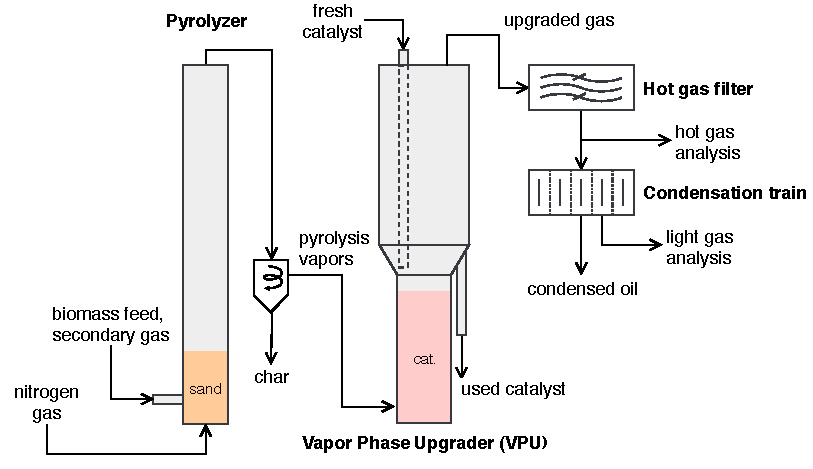
\includegraphics[width=\textwidth]{system.pdf}
    \caption{Overview of the NREL 2FBR system. Biomass fast pyrolysis occurs in the pyrolyzer (left) and gaseous products are catalytically upgraded in the vapor phase upgrader (right).}
    \label{fig:nrel-system}
\end{figure}

\begin{figure}[ht]
    \centering
    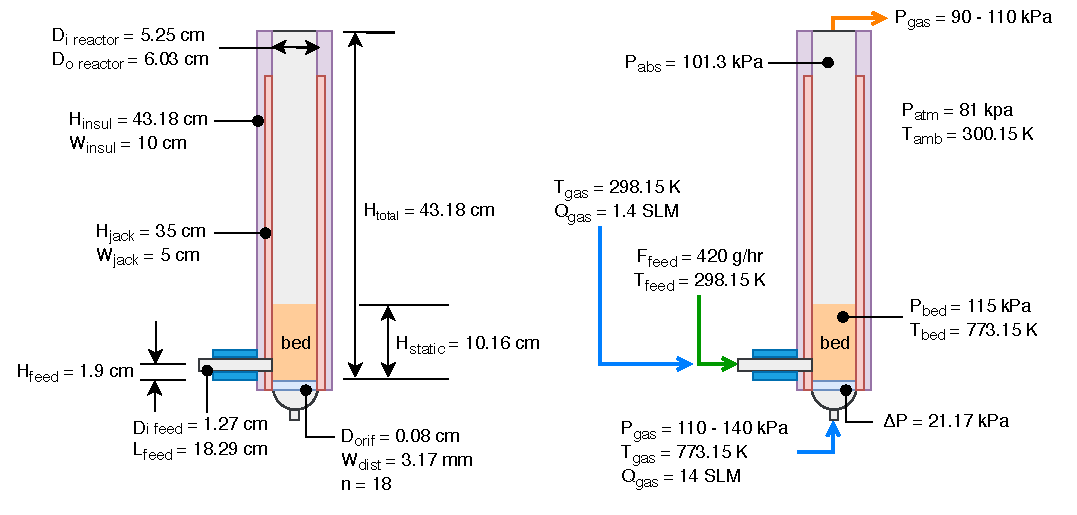
\includegraphics[width=\textwidth]{pyrolyzer.pdf}
    \caption{Dimensions and typical fast pyrolysis operating conditions of the NREL 2FBR pyrolyzer.}
    \label{fig:nrel-pyrolyzer}
\end{figure}
